\section{Server architecture}
The server is implemented in Dropwizard, which is a framework to make RESTful web services. The team chose a RESTful approach because it makes the server easier to interface with as it is stateless. The data-interchange format chosen to transfer data between the app and the server is JSON. This format was chosen for its human readability and it is also very easily parsed by computer software.

The server exposes a set of endpoints that will have a behavior when a HTTP (GET, PUT etc.) request is sent to it. These endpoints provide all the functionality of the server like syncing of data and fetching friend activity. The main structure of how the server uses resources and the database can be found in figure~\ref{fig:classDiagramServer}. The main server service creates instances of the resources. When a resource handles a HTTP request will access the database through the ServerDAO (Server Data Access Object). The Dropwizard implementation that is used makes it very easy to handle requests and send data. A set of resources are defined that and each endpoint will bind to a method in a resource. An example implementation of a resource is included in the source code \hyperref[lst:dropwizardResource]{below}. The resource class and methods are annotated with parameters such as path and HTTP request type. The path can also contain variables so data can be passed to the server directly in the URI. 

The data is stored in a MySQL database using the JDBC API and JDBI for easier interfacing. A diagram of how the database is designed can be found in figure~\ref{fig:ER-Diagram}


\begin{lstlisting}[language=java, frame=single, breaklines=true, caption={Dropwizard resource example}, label={lst:dropwizardResource}]
@Path("user/{user}/sync")
@Produces(MediaType.APPLICATION_JSON)
public class SyncResource {
    @GET
    @Path("/usage/{timestamp}")
    public List<DeviceUsage> getUpdatedUsage(
	   @PathParam("timestamp") LongParam timestamp, 
	   @PathParam("user") LongParam userId) {
        List<DeviceUsage> usage = db.getUpdatedUsage(
		       userId.get(), timestamp.get());
        if(usage != null && !usage.isEmpty())
            return usage;
        else
            throw new WebApplicationException(
			         Response.Status.NO_CONTENT);
    }
}
\end{lstlisting}

\begin{figure}[H]
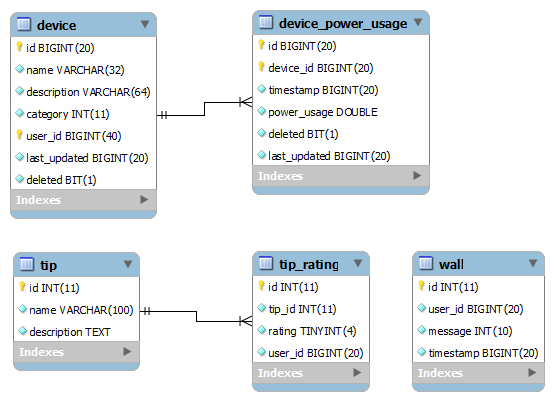
\includegraphics[width=\textwidth]{ch/architecture/fig/ER-Diagram.png}
\caption{ER-Diagram for the database}
\label{fig:ER-Diagram}
\end{figure}

\begin{figure}[H]
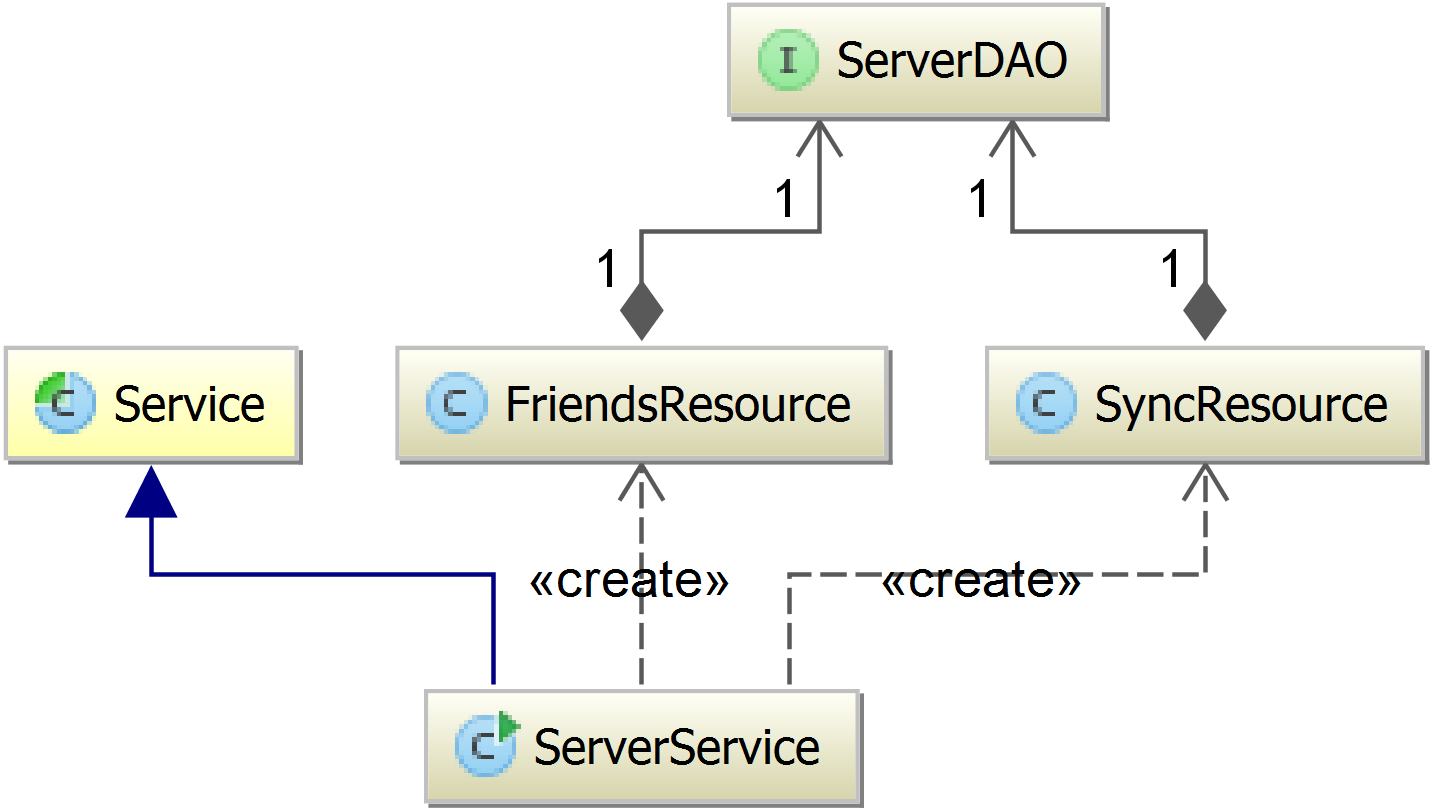
\includegraphics[width=\textwidth]{ch/architecture/fig/classDiagramServer.png}
\caption{Class diagram for main server structure}
\label{fig:classDiagramServer}
\end{figure}